\subsubsection{Modelado de Yair Marin} % (fold)
\label{ssub:ModeladodeYairMarin}
    El algoritmo utilizado para modelar el comportamiento del \textit{Physarum Polycephalum} 
        en el documento se basa en aut\'omatas celulares y se define por un conjunto de estados 
        y reglas de transici\'on espec\'ificas. Los estados incluyen campo libre, nutriente no 
        encontrado, repelente, punto inicial, gel en contracci\'on, gel con compuesto, 
        nutriente hallado, expansi\'on del \textit{Physarum} y gel sin compuesto. 
        Estos estados evolucionan de acuerdo con la vecindad de von Neumann, que 
        considera las c\'elulas adyacentes en las direcciones norte, sur, este y oeste.
    \vskip 0.5cm
    Las reglas de transici\'on determinan c\'omo cambia el estado de cada c\'elula en funci\'on de 
        sus vecinos. Por ejemplo, una c\'elula en estado de campo libre (q0) puede pasar al 
        estado de expansi\'on del \textit{Physarum} (q7) si est\'a adyacente a un punto inicial 
        (q3), gel en contracci\'on (q4) o nutriente hallado (q6). Del mismo modo, una c\'elula en 
        estado de nutriente no encontrado (q1) cambia a estado de nutriente hallado (q6) si 
        est\'a cerca de un gel con compuesto (q5) o otro nutriente hallado (q6). Estas reglas 
        permiten que el modelo emule el comportamiento del \textit{Physarum} en la b\'usqueda y 
        exploraci\'on de su entorno, formando redes eficientes para el transporte de nutrientes 
        y adapt\'andose a cambios en el entorno \cite{MarinAlavez2018}.
    \vskip 0.5cm
    En la Figura \ref{fig:algorithm_running}, se muestra una ejecuci\'on del algoritmo, demostrando 
        c\'omo el \textit{Physarum} se expande y encuentra nutrientes en un entorno simulado.

    % Imagen del algoritmo corriendo
    \begin{figure}[h]
        \centering
        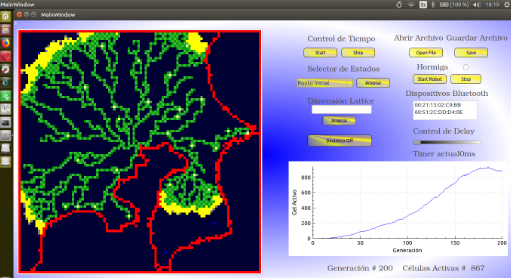
\includegraphics[width=0.7\textwidth]{./images/estado_del_arte/physarum/yahirPrograma.png}
        \caption{Ejecuci\'on del algoritmo de \textit{Physarum Polycephalum} encontrando nutrientes. \cite{MarinAlavez2018}}
        \label{fig:algorithm_running}
    \end{figure}
% subsubsection Modelado de Yahir Marin (end)